\documentclass[12 pt]{article}

\usepackage{enumitem, setspace, listings, graphicx}

\title{Team 22 \\
	Open Bittorrent Directory Replication Final Report}

\author{Adam Howard \\
	\texttt{ahowar31@vols.utk.edu}
	\and
	Maurice Marx \\
	\texttt{mmarx@vols.utk.edu}
	\and
	John Reynolds \\
	\texttt{jreyno40@vols.utk.edu}
	\and
	Jeremy Rogers \\
	\texttt{jroger44@vols.utk.edu}
	\and
	Matthew Seals \\
	\texttt{mseals1@vols.utk.edu}}

\date{April 24, 2015}

\newlist{enum}{enumerate}{6}
\setlist[enum]{label*=\textbf{\arabic*.},leftmargin=*}

\begin{document}
	\maketitle
	\vspace{180 pt}
	Customer: Dr. James S. Plank
	\pagebreak
	\doublespacing
	
	\tableofcontents
	
	\pagebreak
	
	\section{Executive Summary}
	
	The purpose of the Open Bittorrent Directory Replication project is to develop a free alternative to the Bittorrent Sync utility. Bittorrent Sync offers users file replication across multiple computers in a way similar to the widely used Dropbox application, but is built on top of the Bittorrent Protocol, requires no centralized file server, and has no limits on the size of the data that can be stored in it. Our team's goal for the course was to produce the desired software suite and support systems. To help make this goal feasible, we decided to split the project into three main parts: the torrent utility, the tracker, and the configuration tool. The torrent utility can be viewed as the client program for our product. Users may run it as either a foreground or a background process. The tracker is a web server that will keep track of which of the daemons is online, and to communicate to that daemon the locations of its peers. The configuration tool is a script which the user can use to change settings for the utility, such as the login information of the tracker or the directories that need to be monitored. The configuration tool also has a graphical user interface, or GUI, that presents a user-friendly alternative to the command line for changing the Open Bittorrent Directory Replication software settings. As of the time this report was written, the core functionality of all three parts is finished, and the software is to be released under the BSD 3-Clause License.
	
	\pagebreak
	
	\section{Requirements}
	
	\begin{enum}
		\item Definitions (\textit{Taken from http://jonas.nitro.dk/bittorrent/bittorrent-rfc.html})
		\begin{enum}
			\item Peer - A peer is a node in a network participating in file sharing. It can simultaneously act both as a server and a client to other nodes on the network.
			\item Neighboring peers - Peers to which a client has an active point to point TCP connection.
			\item Client - A client is a user agent that acts as a peer on behalf of a user.
			\item Torrent - A torrent is the term for the file (single-file torrent) or group of files (multi-file torrent) that the client is downloading.
			\item Swarm - A network of peers that actively operate on a given torrent.
			\item Seeder - A peer that has a complete copy of a torrent
			\item Tracker - A tracker is a centralized server that holds information about one or more torrents and associated swarms. It functions as a gateway for peers into the swarm.
			\item Metainfo file - A text file that holds information about the torrent, e.g. the URL of the tracker. It usually has the extension .torrent.
		\end{enum}
		\item Utility
		\begin{enum}
			\item Usage
			\begin{enum}
				\item The utility will run as a background process (daemon) on the local system.
				\item The utility will monitor a number of specified directories on the local file system.
				\item The utility will automatically create and modify a Metainfo file (.torrent) for each monitored directory.
				\item The utility will periodically check monitored directories for file modifications by their timestamps.
				\item The utility will inform peers when a modification occurs in one of its monitored directories by distributing an updated version of its Metainfo file.
				\item The utility will listen for updates from peers, and will modify its monitored directories to reflect that update.
			\end{enum}
			\item Configuration
			\begin{enum}
				\item The utility will have a number of configuration parameters which can be adjusted based on the user's preference.
				\item Configuration parameters will be specified within a text file stored on the local file system.
				\item Networking settings will be defined within the configuration file.
				\item Directories to be monitored by the utility will be defined within the configuration file.
				\item Each directory defined in the configuration file may have a number of parameters defined (required parameters are indicated and optional parameters will be given some default value).
				\begin{enum}
					\item The directory's path on the file system.
					\item An identifier for the directory.
					\item How often the utility should check the directory for updates.
					\item Upload/Download rate limits for transfers to and from the directory
				\end{enum}
			\end{enum}
			\item File Manipulation
			\begin{enum}
				\item The utility will attempt to modify files in the monitored directories, as well as Metainfo files, automatically.
				\item The utility will allow the user to add files within a monitored directory.
				\item The utility will allow the user to remove files within a monitored directory.
				\item The utility will allow the user to rename files within a monitored directory.
				\item The utility will allow the user to modify files within a monitored directory.
			\end{enum}
			\item Network Communication
			\begin{enum}
				\item NAT and Gateway
				\begin{enum}
					\item The utility may automatically choose a port and use Universal Plug and Play (UPnP) to ensure that it is accessible behind a router.
					\item The user may manually define the networking settings if he/she chooses to do so.
				\end{enum}
				\item Tracker
				\begin{enum}
					\item Users may communicate with any trackers they choose for coordinating their swarm of devices.
					\item Security considerations are only guaranteed with any degree of certainty when communicating with tracker services we provide.
					\begin{enum}
						\item No passwords will be stored in plaintext by a service we control.
						\item Communication with the tracker will be encrypted using TLS/SSL.
					\end{enum}
					\item Trackerless operation using Distributed Hash Tables will be supported.
				\end{enum}
				\item Peers
				\begin{enum}
					\item Users will be required to authenticate a new peer to any given client.
					\item Peers will communicate to trade up-to-date versions of the monitored directories' Metainfo files.
					\item File transfer between peers will utilize the Bittorrent Protocol.
				\end{enum}
			\end{enum}
		\end{enum}
		\item Supporting Software and Services
		\begin{enum}
			\item Configuration Tool
			\begin{enum}
				\item The Configuration Tool can be issued commands to start and stop the utility.
				\item The Configuration Tool will provide a command line interface.
				\item The Configuration Tool will modify the text file the utility users for configuration.
				\item The Configuration Tool will allow the user to add to, remove from, or modify the list of monitored directories without modifying the contents of the monitored directories.
			\end{enum}
			\item Application-Specific Private Tracker Service
			\begin{enum}
				\item We will provide users a tracker for instances of the utility to connect to.
				\item The service will provide a web interface for managing the tracker.
				\item The service will require user registration and authentication.
				\item The service will allow users to add or remove monitored directories.
			\end{enum}
		\end{enum}
		\item Standards, Licensing, and Supported Platforms
		\begin{enum}
			\item The software will be published using the BSD 3-Clause License.
			\item The utility will comply with Bittorrent Protocol Version 1.0 (BTP/1.0).
			\item All software components will support deployment on the GNU/Linux operating system.
			\begin{enum}
				\item The Debian distribution and its derivatives will be specifically targeted for support.
			\end{enum}
		\end{enum}
	\end{enum}
	
	\section{Change Log}
	
	The first change that was made to the original project was the name. The first name we had was Bittorrent File Sync, or BTFS. This was changed to Open Bittorrent Directory Replication, or Open BDR. Originally, we had planned to license under GPL, but to keep things simple, we decided on a BSD 3-Clause License instead. 
	
	In the configuration file section of the requirements (or \textbf{2.2.5}), some simple things were changed. The scanning rate for directories was moved be a single, general rate, instead of having one for each directory. Also, upload/download rate limits were not implemented due to time constraints.
	
	At point \textbf{2.4.2.3}, trackerless operation is also not supported due to time constraints.
	
	\section{Design Process}
	
	\subsection{Utility}
	
	The utility can be viewed as the client program for our product. As stated above, it can run as a background or a foreground process. It connects to the swarm via settings specified by the configuration tool. The utility periodically checks the monitored directories for changes. If changes are detected, updated metainfo (.torrent) files are distributed to the tracker. When the utility is launched, the tracker is checked for the most recent metainfo files. If there is an updated metainfo, the utility will download the metainfo and modify the related monitored directory to reflect the change. There is a one-to-one correlation between monitored directories and the number of metainfo files. In addition to checking the tracker for updated metainfo files at client startup, the utility performs the same check periodically throughout the program's execution on a time interval, which is by default, 60 seconds. This interval can be modified via the configuration tool.
	
	The utility is implemented in the C++ programming language. It configures itself by reading the configuration file created by the configuration tool. The bittorrent capabilities are provided by the open-source library \texttt{libtorrent}. This library provides features such as torrent downloading automatically when given a torrent file. The library reads the metainfo file, connects to the tracker to find peers, and then downloads all of the pieces of the specified files from the swarm. This proved to be an incredibly useful library for our purposes. Further, it was able to create a metainfo file given a directory. This aided in the code writing process for synchronizing peers, as we did not have to write any code to create standard compliant metainfo files. The bulk of the software that we wrote was monitoring the directories and communicating with the tracker via THP, or Tracker HTTP Protocol, to stay synchronized with the swarm's peers. Authentication with the tracker is achieved via a user's \texttt{peer\_id}. Authentication is required for communication with the tracker. This means that an unauthenticated user's utility is unable to update a metainfo file, download a metainfo file, or download a peer list for a metainfo file. The \texttt{libtorrent} library provided all of the Peer Wire Protocol, or PWP, bittorrent functionality, and thus left our team with more time to make our client feature-rich.
	
	The utility is able to support directory monitoring for a directory in any given location within the file system on a user's computer. When adding a directory through the configuration tool, the location is chosen, and that is recorded in the configuration file. The utility determines the following by simply parsing the configuration file: directory path, directory name, and the rate at which the directory should be scanned to check for modifications. Once a metainfo file is shared with the tracker, a peer is able to discover changes for the related monitored directory. The utility automatically modifies or creates files in monitored directories to remain synced with the directory's most recent metainfo file. Furthermore, if a monitored directory is changed by a user, the utility will notice this during either routine scans specified by the configuration file or by the initial launch scan. If a change is detected, \texttt{libtorrent} is used to create an updated metainfo file. The updated file is then uploaded to the tracker in order to share the changes with the swarm's peers. It is at this point that the updated metainfo file will be noticed by other peers performing routine checks, as it is a part of these routine checks to connect to the tracker and check for updates to the monitored directories. Changes are detected using the \texttt{inotify} API. This API allows for the initialization of an event queue given directories, where the event queues will be filled with events related to changes made in or to the specified directories. The \texttt{inotify} event queues default to a capacity of 16,384 events, which means that the event queue could potentially experience overflow. Because of this, the utility checks the event queues at a default rate and moves events into a buffer. The scanning rate specified in the configuration file is used to check the buffer for updates to the directories represented by metainfo files. This means that the event queue is checked for events at a shorter time interval than the updating of metainfo files, which helps to prevent overflows of the event queue and removes the requirement that the metainfo file update loop must now check the event queue. Now it must simply check the buffer, and thus will already know whether an update is necessary or not.
	
	The utility is easy to launch and acts autonomously using the configuration file for its initial settings. The utility synchronizes a user's directories by communicating with the tracker to obtain a peer list and then downloading the files from the other peers in the swarm. Users are able to easily maintain a standard workspace for whatever purpose they need by simply configuring and launching a utility process on each machine that participates in the swarm. This type of replication provides an inherent fault tolerance, as lost data on a single machine can simply be recovered from the peers also found in the swarm.
	
	\subsection{Tracker}
	
	To manage the daemons, a server was needed that would keep track of which of the daemons is online and to communicate to that daemon the locations of its peers. This server is referred to as a tracker and is a webserver that responds to requests from the daemons with an up-to-date list of all the peers it is currently communicating with. In addition to communicating with the daemons, the tracker also needed to allow the user to manage their account and the directories which are monitored and shared between the daemons.
	
	The tracker was developed using Django, a high-level Python web framework. We chose Django because it provides many features that helped to alleviate the tracker design, such as user accounts and automatic form validation. The primary reasons that we chose Django over any alternatives is that it was free and simple to use, and it is published open-source under a BSD license, so it was appropriate for the intended distribution of this project. The tracker application exposes two main ``views:'' that observed by the utility, and that which the user, or the configuration tool acting as the user, contacts to allow and disallow certain peers and to manage which directories are to be monitored. 
	
	Daemons communicate with the tracker over Bencoded HTTP requests and responses. A Bencoded request contains a dictionary of key/value pairs describing the daemon and the directory it is requesting information about. The response contains a list of active peers that the tracker is aware of and that the daemon contacts to attempt to obtain parts of the requested files. It is important to note, that while the tracker maintains the peer information, it does not have the content of any of the files within the directory and does not necessarily know anything about the torrents it manages.
	
	All of the above is defined with the BTP/1.0 standard, but to make the system work, and to ensure security, certain extensions were made. For one, in addition to the normal request/response pairs which provides the daemon with the peer list, the tracker also provides the daemon with an up-to-date copy of the metainfo (.torrent) file that the monitored directory is described in. The daemon will regularly request this file, and either receives a response containing the HTTP status code 304 to indicate that no updates have occurred or a copy of the updated metainfo file provided as a text response. To provide security, and to prevent unauthorized daemons or other unknown clients from accessing the peer list, a record of known identification numbers is kept. Any request for the peer list or metainfo file which does not contain a known identification number receives a response containing the HTTP status code 403 to indicate that the daemon is forbidden from accessing that information, and the sensitive data will not be transmitted.
	
	The tracker also provides services which can be accessed by the user directly. The user maintains an account with the tracker which is used for authentication. Once authenticated, the user is provided with the ability to add, remove, and manage the directories that the daemons can contact the tracker for peer information on. For each of these directories, a list of identification numbers can be managed by the user to enable which daemons can access information about that directory from the tracker. The configuration tool can act as the user in communicating with the tracker to manage the directory listings and the list of daemons which are able to access each of them.
	
	\subsection{Configuration Tool}
	
	The Configuration Tool is such that we needed to come up with a configuration file structure that was not only easily human-readable, but also easy to parse from a programming standpoint. Originally, while brainstorming a way to do this, we decided to use an nginx-style structure, as follows.
	
	\lstinputlisting{oldconfig.conf}
	
	This proved to be difficult to read and edit, appeared to be difficult to parse, and also stored the password in plaintext, which is against the requirements. After researching different ways to go about this, we came across the ConfigParser Python library, which creates, modifies, and writes to configuration files of a different format, shown below. Also, this file type still has the old BTFS name instead of the newer Open BDR, which is used in the newer configuration file.
	
	\lstinputlisting{newconfig.conf}
	
	The IDs are blank because they are filled in with the return value from the tracker, and this is a fresh configuration. 
	
	We used Python 3 to implement this tool, since we felt that file I/O and parsing are a strength of a scripting language such as Python. Also, the team members working on this part had previous experience using it.
	
	Originally, the configuration tool consisted of two parts: a first time setup script and a bootstrap script. The setup script was only for first time setup, and it had the user input setting such as the tracker domain, the tracker username, and the directories to be monitored. The bootstrap script was to register the user, the peer, and all of the shares (or directories) with the tracker. This approach was abandoned later in the project for a more customizable approach. With the current style of the script, it can be invoked with \texttt{python openbdr\_config.py [command]}, where ``command'' is some function, such as \texttt{addshare, setuser, registeruser}, etc. This was to give the user more control over the configuration tool and to make writing the GUI easier.
	
	The other part of the configuration tool is the graphical user interface, or GUI. For this, we chose to use the Qt framework to implement this part. We chose Qt for a number of reasons, but the main ones being ease of use and familiarity. Qt is easy to use thanks to its language, which is C++ combined with QML, Qt's proprietary language. Since the team has experience in C++, QML was not a problem to learn. The Qt application shows the options that can be edited with the configuration tool and will edit them appropriately. Below is a mock-up of the GUI.
	
	\begin{center}
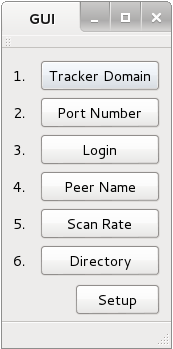
\includegraphics[width=0.4\linewidth]{GUI}
\end{center}

	
	\section{Lessons Learned}
	
	In actuality, there was only one major unexpected event in working on this project. The \texttt{libtorrent} library is a vastly complicated and useful tool. Because of the complexity, the software has many different modules important to development. The time estimated for successful project integration was not a good estimation, and the process ended up requiring longer than initially expected. A minor problem we had was that the previous configuration tool wasn't fully user friendly or able to dynamically change the configuration file. This was adapted to by rewriting the configuration tool in a more CLI-friendly way.
	
	There were many useful things that we learned in doing this project. For one, learning how to use different APIs, such as Django, \texttt{libtorrent}, and Qt, taught us not only how to use these specific APIs but also prepared us for using other APIs in our future careers. We also learned how to divide a large project up into manageable parts and how to work as a team to finish these parts in a timely manner.
	
	As one can see from the change log above, almost all of the functionality that we planned at the beginning of the project was finished, with only a few minor uses being unfinished due to time. For this reason, we feel that the project was a success.
	
	\section{Contributions}
	Adam served as Team Leader, communicating progress and needs with the TAs and Client as well as worked to coordinate team members to complete course assignments. As Team Librarian, he was also responsible for organizing the team's version control repository, and pushing team members to keep it up to date.
	
	In terms of contributions to the project, he steered the general design approach to the software. Adam was personally responsible for implementing and testing the Tracker due to his experience with the relevant languages and frameworks, and worked to produce modules for the Configuration Tool to use as an interface to the Tracker. Significant time was spent working with the Utility team to ensure that the two pieces of software were interoperable. Finally, in designing the demo, he was responsible for creating the virtual machine appliance which contained a mock-up of a production-ready Tracker as well as several peer machines which would run the Utility. This appliance helped to remove issues with networking and made testing of the Utility much simpler.
	
	Maurice was responsible for implementing the local directory monitoring in the daemon. Whenever a file changes in a directory that is being monitored, the daemon acknowledges the change and takes appropriate action to sync the files among all peers. To implement the directory monitoring he used a Linux API called inotify. Inotify uses an event queue to notify the process of a change in a directory. It provides useful information about the altering of a file in a directory, such as the name of the file and whether the file was modified/added/deleted. The only challenge in using inotify to monitor directories was the fact that it did not do recursive directory monitoring. As a consequence, the complexity of the monitoring was slightly increased because the process of recursively adding or removing files had to be automated. The recursive functionality was implemented using a simple tree data structure that modeled the state of the watched directories.
	
	John helped to develop the utility for OpenBDR alongside Maurice. He used libtorrent, the open-source torrenting library, to handle all bittorrent related requirements. He used libcurl to write code that communicates with the tracker by sending http GET and POST requests. The GET requests are used to download the most up-to-date metainfo file for a given monitored directory. The POST requests are used to upload an updated directory's metainfo file to the tracker. The bulk of his time was spent learning libtorrent and attempting to fix bugs associated with it. He also wrote the configuration parser for the utility, which parses the configuration file created by the configuration tool and sets up the libtorrent session appropriately. The utility's tracker communication is multi-threaded so that conflicts with Maurice's filesystem change monitoring code were avoided. He also helped to edit drafts of the required submitted documents this semester; including this one. Further, he created (with some help) the presentations that we gave in class. He helped to work towards our team's goals in order to see them met by the end of the semester.

Jeremy was responsible for implementing the Python configuration tool and compiling all semester written reports into a coherent format. As the Lead Writer, it was his job to make sure that all papers were all written in a readable format and that they looked professional upon submission. He was chosen for this because of his previous experience in \LaTeX and his writing responsibilities in 401 last semester. For the configuration tool, it was his job to make sure that the configuration tool was user-friendly and was able to send relevant information to the tracker required for setup. The configuration tool ended up having three iterations, because of suggestions from team members and problems with interoperability, and he was responsible for writing each of them.
	
 Matthew's responsibilities and contributions for this semester's project included reviewing the papers for grammatical errors, creating the poster, testing the configuration tool, and creating the graphical user interface using Qt. He volunteered to design the poster because he has previous experience with creating posters. He designed one at his internship at Oak Ridge National Laboratory over the summer, and designed the one for our project in ECE 401 last semester. As for testing the configuration tool, he had to test it because the graphical user interface, or GUI, is a wrapper for the tool. The GUI provides a more user-friendly way to edit the settings of the configuration tool without having to use the command line interface.
 
 \pagebreak
 
 \section{Signatures}
	

\includegraphics[width=0.3\linewidth]{Adamsig}

	\textbf{Adam Howard} \hfill\\

	
\includegraphics[width=0.3\linewidth]{Mauricesig} \\

	\textbf{Maurice Marx} \\

	
\includegraphics[width=0.3\linewidth]{Johnsig}

	\textbf{John Reynolds} \\

	
\includegraphics[width=0.3\linewidth]{Jeremysig}

	\textbf{Jeremy Rogers} \\

	
\includegraphics[width=0.3\linewidth]{Matthewsig}

	\textbf{Matthew Seals} 
\end{document}